%----------------------------------------------------------------------------------------
%	PACKAGES AND THEMES
%----------------------------------------------------------------------------------------
\documentclass[aspectratio=169]{beamer}
\mode<presentation> {

	\usetheme{Boadilla}
}
\definecolor{lmugreen}{RGB}{0, 136, 58}
\usecolortheme[named=lmugreen]{structure}
\usepackage{graphicx} % Allows including images
\usepackage{booktabs} % Allows the use of \toprule, \midrule and \bottomrule in tables
\usepackage[english]{babel}
\usepackage[utf8]{inputenc}
\usepackage{amsmath,amssymb} % math symbols
\usepackage{graphicx}
\usepackage{float}
\usepackage{hyperref} % for URLs
\newcommand{\gray}{\rowcolor[gray]{.90}}
\usepackage{verbatim}
\usepackage{textpos} % logo position
\usepackage[default]{sourcesanspro} % font type
\usepackage{cases} % math cases
% Caption
\usepackage{caption}
\usepackage{tikz}
\usetikzlibrary{shapes.geometric, arrows.meta, positioning, fit, backgrounds}
\DeclareCaptionFont{tiny}{\tiny}
\captionsetup{font=scriptsize,labelfont=scriptsize,justification=centering}
% ToC
\AtBeginSection[]{
	\begin{frame}[noframenumbering, plain]
	\frametitle{Outline}
	\setcounter{tocdepth}{1}
	\tableofcontents[currentsection]
\end{frame}
}
% Remove navigation
\beamertemplatenavigationsymbolsempty
% R
\usepackage{listings}
\lstset{
language=R,
basicstyle=\scriptsize\ttfamily,
commentstyle=\ttfamily\color{gray},
backgroundcolor=\color{white},
showspaces=false,
showstringspaces=false,
showtabs=false,
tabsize=2,
captionpos=b,
breaklines=false,
breakatwhitespace=false,
title=\lstname,
escapeinside={},
keywordstyle={},
morekeywords={},
belowskip = -1.2 \baselineskip,
}
%----------------------------------------------------------------------------------------
%	TITLE PAGE
%----------------------------------------------------------------------------------------
\addtobeamertemplate{frametitle}{}{%
	\begin{textblock*}{100mm}(0.88\textwidth,-0.5cm)
		\includegraphics[height=1cm,width=2cm]{figures/lmu_logo}
\end{textblock*}}
\title{Side Constraints in Microgrid Dispatch}
\author{Tim, Sarah, Paul, Anton}
\institute[]{}
\date{16.06.2026}
\begin{document}
{
\usebackgroundtemplate{\includegraphics[width=\paperwidth]{figures/lmu-background.pdf}}
\begin{frame}
\begin{columns}
	\begin{column}{0.4\textwidth}
		\vspace{2cm}

		\textbf{\textcolor{white}{\Large Microgrid Dispatch Optimization: Rolling Horizon, Soft-Peak Commit \& Side Constraints }}

		\textbf{\textcolor{white}{\large }}
		\vspace{1cm}

		\textcolor{white}{\footnotesize Tim Knudsen, Sarah Ewerling, Paul Felkner, Anton Hantschmann  \\
        \vspace{0.5cm}
			QCP Practical \\
			16.06.2026}
	\end{column}
	\begin{column}{0.57\textwidth}
		\vspace{1.56cm}
		\begin{center}
			\includegraphics[width=1\textwidth]{figures/lmu_grey.jpg}
		\end{center}
	\end{column}
\end{columns}
\end{frame}
}
%----------------------------------------------------------------------------------------
%	PRESENTATION SLIDES
%----------------------------------------------------------------------------------------

\section{Problem Statement}
%----------------------------------------------------------------------------------------
%	PROBLEM 1 - Components, Variables, Objective
%----------------------------------------------------------------------------------------

\begin{frame}{Microgrid Setup and Objective}

\begin{columns}[t]
\begin{column}{0.46\textwidth}

\begin{block}{Components}
\footnotesize
\begin{itemize}
    \item Energy consumer
    \item Utility grid connection
    \item Photovoltaic system (PV)
    \item Battery Energy Storage System (BESS)
\end{itemize}
\end{block}
\end{column}

\hspace{0.04\textwidth}

\begin{column}{0.46\textwidth}
\begin{block}{Variables}
\footnotesize
\begin{itemize}
    \item Forecasted \textbf{consumer load}
    \item Forecasted \textbf{PV generation}
    \item \textbf{Grid costs} (electricity import, peak charge)
    \item \textbf{Grid revenue} (electricity export)
    \item \textbf{Grid availability}
    \item BESS \textbf{capacity}
    \item BESS \textbf{state of charge (SoC)}
\end{itemize}
\end{block}
\end{column}
\end{columns}
\vspace{0.25cm}
\begin{block}{Objective}
\footnotesize
Minimize total energy cost, taking resiliency revenue into account
\end{block}
\end{frame}

%----------------------------------------------------------------------------------------
%	PROBLEM 2 - Short Summary - Planned Approach
%----------------------------------------------------------------------------------------

\begin{frame}{}

\begin{block}{Planned Approach}
\footnotesize
\begin{itemize}
    \item Use a \textbf{rolling horizon} with a three day window
    \item Operate with a \textbf{soft, adjustable peak}
    \item Solve \textbf{window-by-window} and carry SoC + running peak forwards
    \item Pay an \textbf{additional penalty} if the peak is exceeded
    \item Exceeding the peak in the current month raises the committed peak in the next month
\end{itemize}
\end{block}
    

\vspace{0.2cm}

\centering
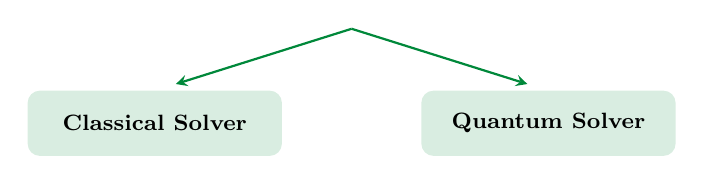
\begin{tikzpicture}[>=stealth, node distance=1.2cm]
  \coordinate (start) at (0,0);

  % Target boxes
  \node (classical) [draw=lmugreen!15, fill=lmugreen!15, thick, rounded corners, minimum width=3.2cm, minimum height=0.8cm] 
    at (-2.5, -1.2) {\footnotesize\textbf{Classical Solver}};
    
  \node (quantum) [draw=lmugreen!15, fill=lmugreen!15, thick, rounded corners, minimum width=3.2cm, minimum height=0.8cm] 
    at (2.5, -1.2) {\footnotesize\textbf{Quantum Solver}};
    
  \draw[->, thick, lmugreen, shorten >= 8pt] (start) -- (classical.north);
  \draw[->, thick, lmugreen, shorten >= 8pt] (start) -- (quantum.north);

\end{tikzpicture}

\end{frame}

\section{MILP $\to$ QUBO Transformation}

% ---------------------------------------------------------------------
% QUBO — what is it?
% ---------------------------------------------------------------------
\begin{frame}{What is QUBO?}
\begin{block}{Quadratic Unconstrained Binary Optimization}
\[
\min_{\mathbf{x}\in\{0,1\}^n}\; \mathbf{x}^\top Q\,\mathbf{x}
\;=\; \sum_i Q_{ii}\,x_i \;+\; \sum_{i<j} Q_{ij}\,x_i x_j \;+\; \text{const}
\]
\end{block}
\vspace{0.2cm}
\begin{columns}[t]
\begin{column}{0.48\textwidth}
\begin{block}{Key properties}
\footnotesize
\begin{itemize}
    \item Only \textbf{binary} variables $x_i\in\{0,1\}$
    \item Only \textbf{quadratic} interactions (at most two variables per term)
    \item \textbf{No explicit constraints} — all constraints folded into the
          objective as \emph{penalty terms}
\end{itemize}
\end{block}
\end{column}
\begin{column}{0.48\textwidth}
\begin{block}{Why relevant?}
\footnotesize
\begin{itemize}
    \item Native format for \textbf{D-Wave quantum annealers} and
          simulated annealing
    \item A violated constraint adds positive energy $\Rightarrow$ annealer
          naturally seeks feasible solutions
    \item Penalty weights $\lambda$ must exceed the max possible objective
          gain from any single violation
\end{itemize}
\end{block}
\end{column}
\end{columns}
\end{frame}

% ---------------------------------------------------------------------
% QUBO — 5 steps overview
% ---------------------------------------------------------------------
\begin{frame}{Five Steps: MILP $\to$ QUBO}
\footnotesize
\begin{enumerate}
    \item \textbf{Binary-encode continuous variables} \\[2pt]
          $v \in [0, v_{\max}] \;\longmapsto\;
           v = \tfrac{v_{\max}}{2^k-1}\sum_{i=0}^{k-1}2^i x_i$
          \hfill Box bounds (B.3) satisfied \emph{by construction.}

    \vspace{0.4em}
    \item \textbf{Equalities $\to$ quadratic penalty} \\[2pt]
          $\textstyle\sum a_i x_i + c = 0
           \;\longmapsto\; \lambda\bigl(\sum a_i x_i + c\bigr)^2$
          \hfill (B.1 balance, B.2 SoC dynamics)

    \vspace{0.4em}
    \item \textbf{Inequalities $\to$ Unbalanced Penalization} \alert{(no slack vars!)} \\[2pt]
          $h(\mathbf{x})\le 0
           \;\longmapsto\; \lambda_1\,h + \lambda_2\,h^2$
          \hfill (B.4 peak coupling, B.5 derating)

    \vspace{0.4em}
    \item \textbf{XOR constraints $\to$ product penalty} \\[2pt]
          $P^{\text{ch}}\cdot P^{\text{dis}} = 0
           \;\longmapsto\; \lambda\,P^{\text{ch}}(\mathbf{x})\cdot P^{\text{dis}}(\mathbf{x})$
          \hfill (B.6 dis-charge)

    \vspace{0.4em}
    \item \textbf{Linear objective $\to$ QUBO diagonal} \\[2pt]
          $c^{\text{ToU}}_t P^{\text{imp}}_t \Delta t
           \;\longmapsto\; \textstyle\sum_i c^{\text{ToU}}_t \Delta t \cdot \mathrm{coeff}_i\, x_i$
\end{enumerate}
\end{frame}

% ---------------------------------------------------------------------
% QUBO — Variable count and qubit requirements
% ---------------------------------------------------------------------
\begin{frame}{QUBO Size: Variables, Bits \& Qubit Requirements}
\begin{columns}[t]
\begin{column}{0.50\textwidth}
\begin{block}{Binary variables per time slot $t$}
\scriptsize
\begin{tabular}{lcc}
\toprule
Variable & \# & bits \\
\midrule
Grid import $P^{\text{imp}}_t$    & 1 & $k_g$ \\
Grid export $P^{\text{exp}}_t$    & 1 & $k_g$ \\
BESS charge $P^{\text{ch}}_t$     & 1 & $k_b$ \\
BESS discharge $P^{\text{dis}}_t$ & 1 & $k_b$ \\
State of charge $E_t$             & 1 & $k_s$ \\
SoC-band indicators $b^{\mathrm{low/mid/high}}_t$ & 3 & 1 ea. \\
\midrule
Peak $P^{\text{peak}}$ \emph{(global)} & 1 & $k_g$ \\
\bottomrule
\end{tabular}
\[
n \;=\; T\cdot\bigl(2k_g + 2k_b + k_s + 3\bigr) + k_g
\]
\end{block}
\end{column}
\begin{column}{0.46\textwidth}
\begin{block}{Runs \& Sweeps (Simulated Annealing)}
\footnotesize
\begin{itemize}
    \item \textbf{Sweep}: visit all $n$ variables once, each flip evaluated in $\mathcal{O}(\deg)$
    \item \textbf{Run}: $S$ sweeps from one random start $\rightarrow$ one candidate solution
    \item $R$ independent runs $\rightarrow$ best sample kept
\end{itemize}
\vspace{0.3em}
\textbf{Runtime:}
\[
\mathcal{O}(R\cdot S\cdot n^2)
\]
Dense $Q$: $\deg \approx n$ (all-to-all interactions). \\
Our model: sparse $Q$ ($\deg \propto k$) $\Rightarrow \mathcal{O}(R\cdot S\cdot n\cdot k)$.\\[0.4em]
\textbf{Consequence:} $n \uparrow$ harms \emph{quadratically} for dense problems — fewer bits $k$ reduces $n$ and speeds up solving.
\end{block}
\vspace{0.15cm}
\begin{block}{Example: $k_g\!=\!k_b\!=\!k_s\!=\!4,\;T\!=\!24$ slots}
\footnotesize
$n = 24\cdot(8+8+4+3)+4 = \mathbf{556}$ variables
\end{block}
\end{column}
\end{columns}
\vspace{0.1cm}
{\footnotesize\centering
Each continuous variable uses $k$ bits $\Rightarrow$ resolution $= v_{\max}/(2^k-1)$;
off-diagonal $Q_{ij}$ entries encode interactions between bits of \emph{different} variables.\par}
\end{frame}

% ---------------------------------------------------------------------
% QUBO — full objective
% ---------------------------------------------------------------------
\begin{frame}{The Resulting QUBO Objective}
\scriptsize
\[
\min_{\mathbf{x}}\;
\underbrace{
  \sum_t c^{\text{ToU}}_t P^{\text{imp}}_t \Delta t
  - \sum_t c^{\text{exp}} P^{\text{exp}}_t \Delta t
  + c^{\text{dem}} P^{\text{peak}}
  - \sum_{t\in\mathcal{O}} r^{\text{res}} y_t
}_{\text{energy cost + demand charge + export revenue + resilience reward}}
\]
\vspace{-0.5em}
\[
+\;
\underbrace{
  \lambda_{\text{bal}}\sum_{t:\,g_t=1}
  \bigl(P^{\text{PV}}_t + P^{\text{imp}}_t - P^{\text{exp}}_t
        + P^{\text{dis}}_t - P^{\text{ch}}_t - P^{\text{load}}_t\bigr)^2
}_{\text{power balance penalty}}
\]
\vspace{-0.5em}
\[
+\;
\underbrace{
  \lambda_{\text{soc}}\sum_t
  \bigl(E_t - E_{t-1} - \eta\,P^{\text{ch}}_t\,\Delta t
        + \tfrac{\Delta t}{\eta}\,P^{\text{dis}}_t\bigr)^2
}_{\text{SoC dynamics penalty}}
\;+\;
\underbrace{\sum_t\bigl[\lambda_1 h^{\text{pk}}_t + \lambda_2 (h^{\text{pk}}_t)^2\bigr]}_{\text{peak coupling (unbalanced pen.)}}
\]
\vspace{-0.5em}
\[
+\;
\underbrace{\lambda_{\text{xor}}\sum_t \bigl(P^{\text{ch}}_t P^{\text{dis}}_t
  + P^{\text{imp}}_t P^{\text{exp}}_t\bigr)}_{\text{charge/discharge \& import/export XOR penalty}}
\;+\;
\underbrace{\sum_t\bigl[\lambda_1 h^{\text{der}}_t + \lambda_2 (h^{\text{der}}_t)^2\bigr]}_{\text{SoC-band power derating (unbalanced pen.)}}
\]
\vspace{-0.5em}
\[
+\;
\underbrace{
  \lambda_{\text{b7}}\!\sum_{t\in\mathcal{O}}\!\Bigl[
    \bigl(m_t(1{-}y_t) - \bar{P}_t - s_t^{\uparrow}\bigr)^2
    +\,\bigl(m_t(1{-}y_t) + \bar{P}_t - s_t^{\downarrow}\bigr)^2
  \Bigr]
}_{\text{outage island balance: } |\bar{P}_t|\le m_t(1-y_t),\text{ i.e.\ exact balance iff load served } (y_t=1)}
\]
\vspace{0.1cm}
\begin{itemize}
    \item $h^{\text{pk}}_t = P^{\text{imp}}_t - P^{\text{peak}}$,\quad
          $h^{\text{der}}_t = P^{\text{ch/dis}}_t - \tfrac{1}{2}P^{\text{B}}_{\text{nom}}(1+b^{\text{mid}}_t)$,\quad
          $\bar{P}_t = P^{\text{dis}}_t - P^{\text{ch}}_t + P^{\text{PV}}_t - P^{\text{load}}_t$
    \item $\lambda$ auto-scaled: $\lambda \ge 2\times\max_i Q_{ii}^{\text{obj}}$
          \small(Bak\'{o} et al.\ 2025, Eq.~1)
    \item All variables binary-encoded (Step 1) $\Rightarrow$ B.3 holds by construction
\end{itemize}
\end{frame}

\section{Approach Evolution}

% ---------------------------------------------------------------------
% EVOLUTION 1 — feedback -> changes
% ---------------------------------------------------------------------
\begin{frame}{How the Approach Evolved (Feedback $\rightarrow$ Now)}
\begin{block}{Last session's feedback: the real billing}
\footnotesize
You \textbf{commit} a peak in advance, \textbf{pay a penalty} if you exceed it, and a
\textbf{higher peak is set next month}; you operate as the month actually unfolds.
\end{block}
\begin{columns}[t]
\begin{column}{0.46\textwidth}
\begin{block}{Before}
\footnotesize
\begin{itemize}
    \item One solve over the whole horizon
    \item A single \textbf{hard} peak: can never be exceeded
    \item Assumes the month is known up front
\end{itemize}
\end{block}
\end{column}
\hspace{0.04\textwidth}
\begin{column}{0.46\textwidth}
\begin{block}{Now}
\footnotesize
\begin{itemize}
    \item \textbf{Rolling horizon}: solve window-by-window, carry SoC $+$ running peak forward
    \item \textbf{Soft peak $+$ penalty}: always pay for the committed peak; pay an \emph{extra} penalty only if you exceed it
    \item \textbf{Ratchet}: exceeding raises next month's committed peak
\end{itemize}
\end{block}
\end{column}
\end{columns}
\vspace{0.15cm}
{\footnotesize\centering Same model core: now it matches how the customer is actually billed.\par}
\end{frame}

% ---------------------------------------------------------------------
% EVOLUTION 2 — objective: last week vs this week
% ---------------------------------------------------------------------
\begin{frame}{Objective Function: Last Week $\rightarrow$ This Week}
\begin{block}{Previous: a single \emph{hard} peak}
\small
\[
\min\ \sum_{t} c^{\text{ToU}}_t P^{\text{imp}}_t \Delta t
\;+\; \alert{c^{\text{dem}}\, P^{\text{peak}}}
\;-\; \sum_{t\in\mathcal{O}} r^{\text{res}} y_t
\]
\end{block}
\begin{block}{Now: committed peak $+$ exceedance penalty}
\small
\[
\begin{aligned}
\min\ &\sum_{t} c^{\text{ToU}}_t P^{\text{imp}}_t \Delta t
\;+\; \alert{c^{\text{dem}}\, P^{\text{commit}} + c^{\text{pen}}\,\bigl(P^{\text{real}} - P^{\text{commit}}\bigr)^{+}} \\
&-\; \sum_{t\in\mathcal{O}} r^{\text{res}} y_t
\;-\; \sum_{t} c^{\text{exp}} P^{\text{exp}}_t \Delta t
\end{aligned}
\]
\end{block}
\begin{itemize}\footnotesize
    \item The one hard-peak term splits into \textbf{committed capacity}
          ($c^{\text{dem}}P^{\text{commit}}$, \emph{always paid}) $+$ a
          \textbf{penalty on exceedance} \big($(x)^{+}=\max(0,x)$\big).
    \item Ratchet: next month's $P^{\text{commit}} \leftarrow \max(P^{\text{commit}}, P^{\text{real}})$.
          \quad (Also new: export revenue $-\,c^{\text{exp}}P^{\text{exp}}$.)
\end{itemize}
\end{frame}

% ---------------------------------------------------------------------
% EVOLUTION 3 — simple rolling-horizon schematic
% ---------------------------------------------------------------------
\begin{frame}{The Rolling-Horizon Idea (One Month)}
\centering
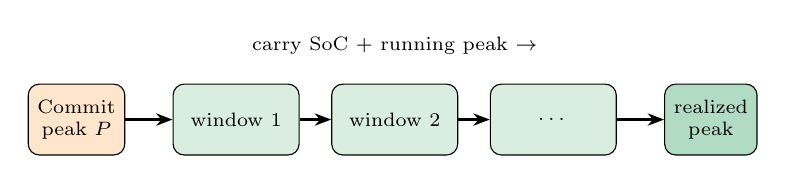
\begin{tikzpicture}[
    win/.style={draw, rounded corners, fill=lmugreen!15, minimum height=0.9cm, minimum width=1.6cm, align=center, font=\scriptsize},
    box/.style={draw, rounded corners, minimum height=0.9cm, align=center, font=\scriptsize},
    arr/.style={-{Stealth[scale=0.9]}, thick}
]
    \node[box, fill=orange!20] (commit) {Commit\\peak $P$};
    \node[win, right=0.6cm of commit] (w1) {window 1};
    \node[win, right=0.4cm of w1] (w2) {window 2};
    \node[win, right=0.4cm of w2] (w3) {$\dots$};
    \node[box, fill=lmugreen!30, right=0.6cm of w3] (real) {realized\\peak};
    \draw[arr] (commit) -- (w1);
    \draw[arr] (w1) -- (w2);
    \draw[arr] (w2) -- (w3);
    \draw[arr] (w3) -- (real);
    \node[font=\scriptsize, above=0.25cm of w2] {carry SoC $+$ running peak $\rightarrow$};
\end{tikzpicture}
\vspace{0.4cm}
\begin{itemize}\footnotesize
    \item \textbf{During the month:} a \textbf{penalty} is charged if the realized peak exceeds $P$
    \item \textbf{End of month:} the \textbf{ratchet} sets next month's commitment $=\max(P,\ \text{realized peak})$
\end{itemize}
\end{frame}


\section{Side Constraints: Two Definitions}

% ---------------------------------------------------------------------
% SIDE CONSTRAINTS — the two definitions
% ---------------------------------------------------------------------
\begin{frame}{Two Ways to Define a ``Side Constraint''}
\begin{columns}[t]
\begin{column}{0.48\textwidth}
\begin{block}{(A) Informal: by role}
\footnotesize
A constraint that \emph{refines} the model rather than stating its physics.
\begin{itemize}
    \item \textbf{Main}: the physical laws that make a solution valid
    \item \textbf{Side}: device limits, economics, modeling hygiene
\end{itemize}
\textit{Question it asks:} ``how fundamental is it?''
\end{block}
\end{column}
\begin{column}{0.48\textwidth}
\begin{block}{(B) Formal: complicating constraint}
\footnotesize
A constraint that \emph{breaks an otherwise clean, fast-to-solve structure}
(Lagrangian / Dantzig--Wolfe / Benders sense).
\begin{itemize}
    \item \textbf{Core}: a special, easy block (e.g.\ network flow)
    \item \textbf{Side}: what destroys that structure or links the blocks
\end{itemize}
\textit{Question it asks:} ``does it make the problem harder to solve?''
\end{block}
\end{column}
\end{columns}
\vspace{0.2cm}
\footnotesize
\centering
Same constraints, different lens: nearly the same split, but different reasoning.
\end{frame}

% ---------------------------------------------------------------------
% SIDE CONSTRAINTS — classification comparison (microgrid MILP)
% ---------------------------------------------------------------------
\begin{frame}{What Counts as ``Side'': Microgrid Dispatch MILP}
\centering
\scriptsize
\begin{tabular}{lcc}
\toprule
Constraint & (A) Informal & (B) Formal \\
\midrule
Power balance                       & main (physical law) & core \\
Battery SoC dynamics                & main (physical law) & core \\
Variable bounds                     & side (capacity)     & \textbf{core} (easy bounds) \\
Peak coupling $P^{\text{peak}}\!\ge\!P^{\text{imp}}$ & side (economics) & \textbf{side: linking} \\
SoC bands / indicators              & side (protection)   & side: integrality \\
Charge/discharge XOR                & side (hygiene)      & side: integrality \\
Import/export XOR                    & side (hygiene)      & side: integrality \\
Outage Big-M $+$ served             & side (resilience)   & side: integrality \\
\bottomrule
\end{tabular}
\vspace{0.3cm}
\begin{itemize}\footnotesize
    \item Partition is \emph{almost} identical, but (B) reclassifies
          \textbf{variable bounds as core}.
    \item (B)'s key insight: the \textbf{peak coupling} is the \emph{linking}
          complication (it ties the scenarios together), a different kind from the
          \textbf{integrality} complications that force branch-and-bound.
\end{itemize}
\end{frame}


\section{The Side Constraints, Formally}

% ---------------------------------------------------------------------
% TYPE 1 (LINKING) — scenario-coupling peak constraint
% ---------------------------------------------------------------------
\begin{frame}{Type 1 (Linking): The Scenario-Coupling Constraint}
\begin{block}{Demand-charge / peak coupling}
\[
P^{\text{peak}} \;\ge\; P^{\text{imp}}_{s,t}
\qquad \forall\, s\in\mathcal{S},\; t\in\mathcal{T}
\]
with $P^{\text{peak}}$ a \textbf{single first-stage variable} (no scenario index).
\end{block}
\begin{itemize}\footnotesize
    \item One shared variable forced $\ge$ \emph{every} import in \emph{every}
          scenario $\Rightarrow$ it equals the worst-case peak over all of them.
    \item \textbf{The only constraint coupling the scenarios:} remove it and the
          $M$ scenarios separate into $M$ independent subproblems.
    \item Gives the program its \textbf{block-angular} structure: the target of
          Benders / Lagrangian decomposition, and what the soft-peak model relaxes
          into a penalty.
\end{itemize}
\end{frame}

% ---------------------------------------------------------------------
% TYPE 2 (INTEGRALITY) — SoC-dependent power bands
% ---------------------------------------------------------------------
\begin{frame}{Type 2 (Integrality): SoC-Dependent Power Bands}
\begin{block}{Band selection, indicators, throttled power}
\begin{align*}
b^{\text{low}}_{s,t} + b^{\text{mid}}_{s,t} + b^{\text{high}}_{s,t} &= 1 \\
b^{\text{low}}_{s,t}=1 &\Rightarrow E_{s,t}\le E^{\text{low}} \\
b^{\text{mid}}_{s,t}=1 &\Rightarrow E^{\text{low}}\le E_{s,t}\le E^{\text{high}} \\
b^{\text{high}}_{s,t}=1 &\Rightarrow E_{s,t}\ge E^{\text{high}} \\
P^{\text{ch}}_{s,t},\,P^{\text{dis}}_{s,t} &\le P^{\text{B}}_{\text{nom}}\big[f^{\text{edge}}(b^{\text{low}}_{s,t}+b^{\text{high}}_{s,t})+f^{\text{mid}}b^{\text{mid}}_{s,t}\big]
\end{align*}
\end{block}
\begin{itemize}\footnotesize
    \item Three binaries select the SoC band; exactly one active per slot.
    \item Power throttled to \textbf{125 kW} at the edges ($f^{\text{edge}}\!=\!0.5$)
          vs.\ \textbf{250 kW} in mid ($f^{\text{mid}}\!=\!1$): battery protection.
    \item \textbf{Why complicating:} the power \emph{bound} now depends on a
          discrete state $\Rightarrow$ no fixed box; the binaries force branch-and-bound.
\end{itemize}
\end{frame}

% ---------------------------------------------------------------------
% TYPE 2 (INTEGRALITY) — XOR mutual exclusion
% ---------------------------------------------------------------------
\begin{frame}{Type 2 (Integrality): Mutual Exclusion (XOR)}
\begin{columns}[t]
\begin{column}{0.46\textwidth}
\begin{block}{Battery: charge XOR discharge}
\[
\begin{aligned}
P^{\text{ch}}_{s,t}  &\le P^{\text{B}}_{\text{nom}}\,b^{\text{ch}}_{s,t}\\
P^{\text{dis}}_{s,t} &\le P^{\text{B}}_{\text{nom}}\,b^{\text{dis}}_{s,t}\\
b^{\text{ch}}_{s,t} + b^{\text{dis}}_{s,t} &\le 1
\end{aligned}
\]
\end{block}
\end{column}
\hspace{0.04\textwidth}
\begin{column}{0.46\textwidth}
\begin{block}{Grid: import XOR export}
\[
\begin{aligned}
P^{\text{imp}}_{s,t} &\le P^{\text{G}}_{\max}\,b^{\text{imp}}_{s,t}\\
P^{\text{exp}}_{s,t} &\le P^{\text{G}}_{\max}\,b^{\text{exp}}_{s,t}\\
b^{\text{imp}}_{s,t} + b^{\text{exp}}_{s,t} &\le 1
\end{aligned}
\]
\end{block}
\end{column}
\end{columns}
\vspace{0.2cm}
\begin{itemize}\footnotesize
    \item Each big constant ($P^{\text{B}}_{\text{nom}}$, $P^{\text{G}}_{\max}$) is a
          \textbf{Big-M} tying the on/off binary to its continuous flow.
    \item \textbf{Formally redundant classically} (efficiency losses already make
          simultaneous charge+discharge uneconomic), but kept to \textbf{mirror the
          QUBO penalty terms}.
\end{itemize}
\end{frame}

% ---------------------------------------------------------------------
% TYPE 2 (INTEGRALITY) — outage Big-M switchable balance
% ---------------------------------------------------------------------
\begin{frame}{Type 2 (Integrality): Outage Handling (Switchable Balance)}
\begin{block}{Conditional island balance (Big-M)}
During an outage ($t\in\mathcal{O}_s$): no grid, $P^{\text{imp}}_{s,t}=P^{\text{exp}}_{s,t}=0$
(bound-fixing, core); the balance becomes switchable:
\[
\big|\,P^{\text{PV}}_{s,t} + P^{\text{dis}}_{s,t} - P^{\text{ch}}_{s,t} - P^{\text{load}}_{s,t}\,\big|
\;\le\; M^{\text{bal}}_{s,t}\,(1 - y_{s,t})
\]
\end{block}
\begin{itemize}\footnotesize
    \item $y_{s,t}=1 \Rightarrow$ RHS $=0$ $\Rightarrow$ the island must balance
          \emph{exactly} (load served, earns resiliency revenue).
    \item $y_{s,t}=0 \Rightarrow$ RHS huge $\Rightarrow$ constraint \emph{off}
          $\Rightarrow$ load shedding allowed, no revenue.
    \item \textbf{Why complicating:} a \textbf{switchable equality} (Big-M $+$ binary
          $y$), the classic disjunction that forces branch-and-bound.
\end{itemize}
\end{frame}


\section{Appendix}

% ---------------------------------------------------------------------
% APPENDIX — block-angular structure & decomposition
% ---------------------------------------------------------------------
\begin{frame}{Appendix: Block-Angular Structure \& Decomposition}
\centering
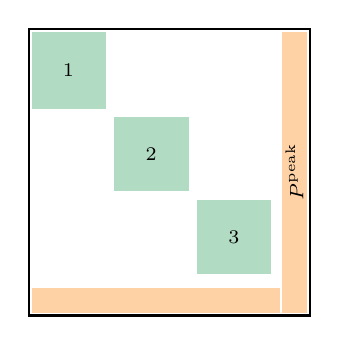
\begin{tikzpicture}[scale=0.7, every node/.style={font=\scriptsize}]
    % outer matrix
    \draw[thick] (0,0) rectangle (5.1,5.2);
    % diagonal scenario blocks
    \fill[lmugreen!30] (0.05,3.75) rectangle (1.4,5.15);
    \fill[lmugreen!30] (1.55,2.25) rectangle (2.9,3.6);
    \fill[lmugreen!30] (3.05,0.75) rectangle (4.4,2.1);
    \node at (0.72,4.45) {1};
    \node at (2.22,2.92) {2};
    \node at (3.72,1.42) {3};
    % linking column (peak)
    \fill[orange!35] (4.6,0.05) rectangle (5.05,5.15);
    \node[rotate=90] at (4.82,2.6) {$P^{\text{peak}}$};
    % linking row (coupling constraints)
    \fill[orange!35] (0.05,0.05) rectangle (4.55,0.5);
\end{tikzpicture}
\vspace{0.25cm}
\begin{itemize}\footnotesize
    \item \textbf{Block-angular}: independent scenario blocks (green, diagonal),
          tied \emph{only} by the orange $P^{\text{peak}}$ row/column, the Type 1
          linking constraint.
    \item \textbf{Benders}: a \emph{master} fixes $P^{\text{peak}}$; each block is
          solved as a \emph{subproblem}; they exchange ``cuts'' until they agree.
    \item \textbf{Lagrangian}: move the linking row into the objective as a
          \emph{penalty} $\Rightarrow$ the blocks separate, exactly what the
          \textbf{QUBO} and the \textbf{soft-peak penalty} already do.
\end{itemize}
\end{frame}


\end{document}
